\documentclass[a4paper, 12pt]{article}
\usepackage[spanish]{babel}
\usepackage[hmargin=2cm,vmargin=2.5cm]{geometry}
\usepackage{enumerate}
\usepackage{makecell}
\usepackage{graphicx}
\usepackage{hyperref}
\usepackage{amsmath}
\usepackage[backend=biber,style=apa, url=true, sortcites]{biblatex}
\usepackage[table]{xcolor}
\usepackage{minted}
\usepackage{graphicx}
\usepackage{fancyhdr}  % Agrega el paquete fancyhdr
\usepackage{subcaption}

\addbibresource{references.bib}
\hypersetup{
	colorlinks,
	citecolor=black,
	filecolor=black,
	linkcolor=black,
	urlcolor=black
}

\setlength{\arrayrulewidth}{0.4mm}

\newcommand{\HRule}{\rule{\linewidth}{0.5mm}}

\begin{document}
    \begin{titlepage}
        \begin{center}
            % logo
            
\includegraphics[width=0.5\textwidth]{figures/logoUAH.png}~\\[2cm]
            
            \textsc{\Large \\Sistemas de Control Inteligente}\\[2cm]
            
            \HRule \\[0.4cm]
            {\LARGE \bfseries Práctica 1. \\ Identificación y control neuronal  \\[0.4cm]}
            \HRule \\[3cm]
            
            \large\textbf{Jorge Revenga Martín de Vidales}\\
            \large\textbf{Ángel Salgado Aldao}\\
            \large\textbf{}\\ Grado en Ingeniería Informática \\ Universidad de Alcalá
            
            \vfill
            
            {\large \today}
        \end{center}
    \end{titlepage}

    % Configura los encabezados y pies de página
    \pagestyle{fancy}
    \fancyhf{} % Limpia todos los encabezados y pies de página actuales
    % Encabezado
    \fancyhead[RO,LE]{\textit{Sistemas de Control Inteligente}}
    \fancyhead[LO,RE]{\textit{Identificación y control neuronal}}  % Encabezado izquierda del documento
    % Pie de página
    \fancyfoot[LO,RE]{\textit{Universidad de Alcalá}}
    \fancyfoot[RO,LE]{\thepage}  % Número de página en la esquina inferior derecha
    \newpage
    
    \thispagestyle{plain}
    \tableofcontents
    \newpage

    \part{}
    
    \section{Ejercicio 1. Perceptrón.}
    
	Se desea clasificar un conjunto de datos pertenecientes a cuatro clases diferentes.       Los datos y las clases a las que pertenecen con los que se muestra a continuación:
 
        \begin{figure}[htp!]
            \centering
            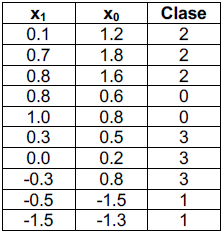
\includegraphics[width=0.25\textwidth]{figures/parte1/Ej1/Ej1_fig0.png}
        \end{figure}

        Se desea diseñar un clasificador neuronal mediante un perceptrón simple que clasifique estos datos. Diseñe el clasificador, visualice los parámetros de la red y dibuje los datos junto con las superficies que los separan.
        
        \subsection{Código}
            \inputminted[fontsize=\scriptsize, linenos, breaklines=true, xleftmargin=0.75cm, frame=lines]{matlab}{code/parte1/Ej1.m}

        \subsection{Preguntas}
        
        \paragraph{¿Consigue la red separar los datos?\\}
            Sí, los clasifica en las 4 clases correctamente
    
        \paragraph{¿Cuántas neuronas tiene la capa de salida?, ¿por qué?\\}
        Tiene 4 neuronas, cada una genera una salida que representa la probabilidad de pertenencia a una clase particular, como tenemos 4 clases, tenemos 4 neuronas

    
        \paragraph{¿Qué ocurre si se incorpora al conjunto un nuevo dato: [0.0 -1.5] de la clase 3?\\}
        Los datos dejan de ser linealmente separables, por loq que las líneas que dividen los datos en las clases dejan de aplicarse a todos los datos, su pendiente ha cambiado pero el nuevo dato no está separado en el mismo espacio que el resto de datos de clase 3. Está con los datos de clase 1

        \newpage
	\subsection{Ejecución}
    	\begin{figure}[htp!]
    		\centering
    		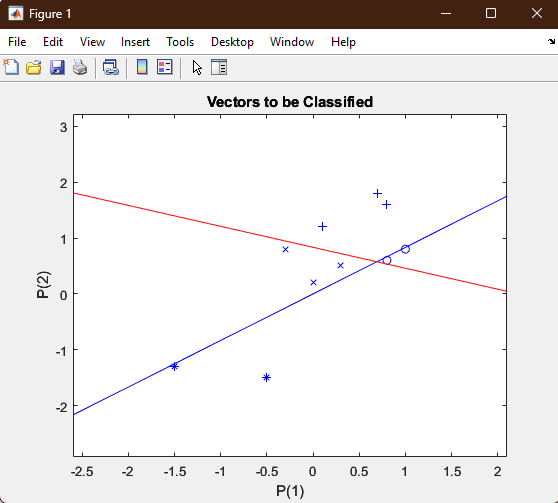
\includegraphics[width=0.69\textwidth]{figures/parte1/Ej1/Ej1_fig1.png}
    		\caption{Ejecución ejercicio 1.}
                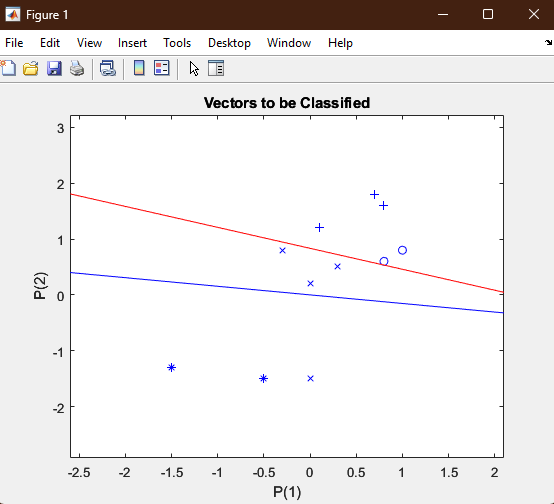
\includegraphics[width=0.69\textwidth]{figures/parte1/Ej1/Ej1_fig2.png}
        		\caption{Ejecución ejercicio 1 con el nuevo dato.}
    	\end{figure}
        \newpage

    
    \section{Ejercicio 2. Aproximación de funciones.}
    
        Una de las aplicaciones inmediatas de las redes neuronales es la aproximación de funciones. Para ello, Matlab dispone de una red optimizada, fitnet, con la que se trabajará en este ejercicio. El objetivo en este caso es aproximar la función \emph{f = sinc(t)} tal y como se muestra a continuación:

        \inputminted[fontsize=\scriptsize, linenos, breaklines=true, xleftmargin=0.75cm, frame=lines]{matlab}{code/parte1/Ej2.m}

        Estudie los efectos sobre la solución final de modificar el método de entrenamiento (consulte la ayuda de Matlab y pruebe 4 métodos diferentes) y el número de neuronas de la capa oculta.

        \subsection{Solución}
            Para poder visualizar el código en funcionamiento primero debemos definir la función \emph{sinc(t)}. Lo haremos en un archivo llamado sinc.m. En nuestro caso hemos definido la siguiente función \emph{sinc(t)}:

            \inputminted[fontsize=\scriptsize, linenos, breaklines=true, xleftmargin=0.75cm, frame=lines]{matlab}{code/parte1/sinc.m}

            Para modificar el método de entrenamiento basta con cambiar el segundo parámetro de la función \texttt{fitnet()} por otra función de entrenamiento, para obtener más información también vamos a cambiar el número de neuronas de la capa oculta de 4 a 8 y comparar el desempeño de cada método de entrenamiento.

            \newpage
            \subsection{Ejecución}
                En el código del enunciado se usa la función 'trainrp', que se refiere a se refiere a 'Resilient Backpropagation'. Este es un método de entrenamiento para redes neuronales que se enfoca en la convergencia rápida mediante la adaptación dinámica de las tasas de aprendizaje para cada peso de la red. Este es su desempeño:
                
                \begin{figure}[htp!]
                    \caption{Resilient Backpropagation}
                    \begin{subfigure}{0.49\textwidth}
                        \centering
        		      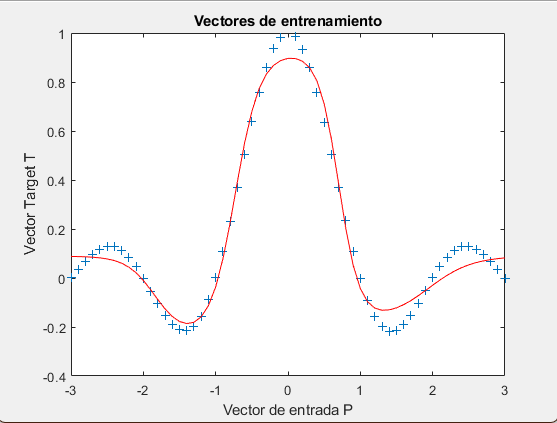
\includegraphics[width=\textwidth]{figures/parte1/Ej2/Ej2_fig0_codigo_enunciado.png}
                        \caption{trainrp con 4 neuronas en capa oculta}
                    \end{subfigure}
                    \begin{subfigure}{0.49\textwidth}
                        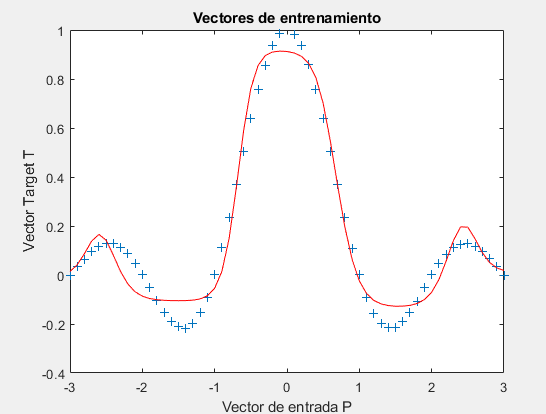
\includegraphics[width=\textwidth]{figures/parte1/Ej2/Ej2_fig9_trainrp_enunciado_8neuronas.png}
                        \caption{trainrp con 8 neuronas en capa oculta}
                    \end{subfigure}
                \end{figure}

            
            \subsection{Entrenamiento con Descenso de Gradiente estándar - 'traingd'}
                Esta función de entrenamiento utiliza el método de descenso de gradiente estándar. Ajusta los pesos de la red en la dirección opuesta al gradiente de la función de costo con respecto a los pesos. Se considera simple y efectivo, pero que puede converger lentamente en algunos casos. En nuestro caso los resultados con 4 y 8 neuronas en la capa oculta no difieren mucho, por lo que se podría decir (con poco rigor) que converge lentamente.

                \begin{figure}[htp!]
                    \caption{Descenso gradiente estándar}
                    \begin{subfigure}{0.49\textwidth}
                        \centering
        		      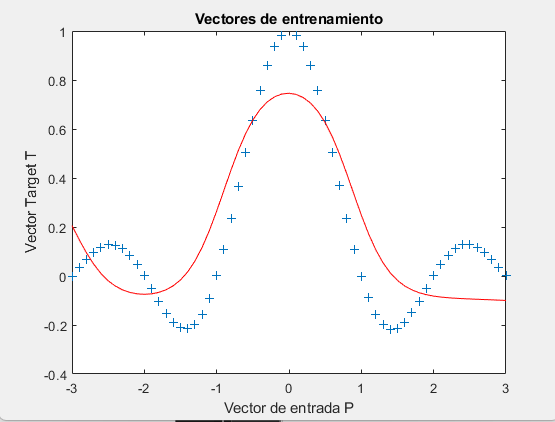
\includegraphics[width=\textwidth]{figures/parte1/Ej2/Ej2_fig1_traingd.png}
                        \caption{traingd con 4 neuronas en capa oculta}
                    \end{subfigure}
                    \begin{subfigure}{0.49\textwidth}
                        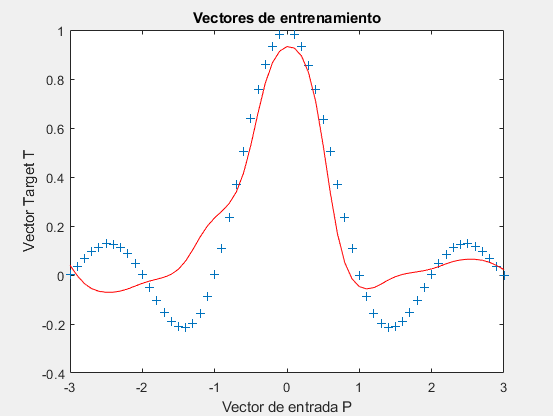
\includegraphics[width=\textwidth]{figures/parte1/Ej2/Ej2_fig5_traingd_8neuronas.png}
                        \caption{traingd con 8 neuronas en capa oculta}
                    \end{subfigure}
                \end{figure}
                
            \subsection{Entrenamiento con Descenso de Gradiente con Momento - 'traingdm' }
                Similar al descenso de gradiente, pero con la adición de "momentum". El momento ayuda a acelerar el entrenamiento al mantener una memoria de las actualizaciones de los pesos anteriores. Teóricamente esto puede ayudar a superar óptimos locales y acelerar la convergencia. Al aumentar el número de neuronas el resultado no muestra mucha mejoría, al igual que el descenso gradiente estándar

                \begin{figure}[htp!]
                    \caption{Descenso gradiente con momento}
                    \begin{subfigure}{0.49\textwidth}
                        \centering
        		      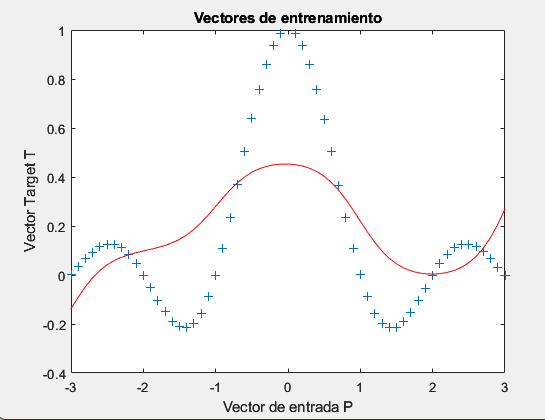
\includegraphics[width=\textwidth]{figures/parte1/Ej2/Ej2_fig2_traingdm.png}
                        \caption{traingdm con 4 neuronas en capa oculta}
                    \end{subfigure}
                    \begin{subfigure}{0.49\textwidth}
                        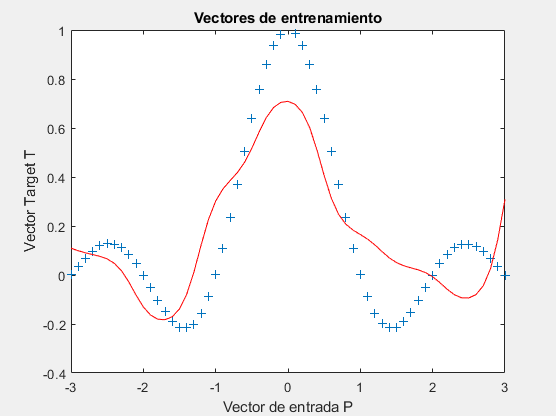
\includegraphics[width=\textwidth]{figures/parte1/Ej2/Ej2_fig6_traingdm_8neuronas.png}
                        \caption{traingdm con 8 neuronas en capa oculta}
                    \end{subfigure}
                \end{figure}

            
            \subsection{Entrenamiento con Levenberg-Marquardt - 'trainlm'}
                Utiliza el algoritmo de Levenberg-Marquardt, que es una técnica de optimización no lineal. Se observa muy buen desempeño con 4 neuronas en la capa oculta y notable mejora al subir a 8 neuronas.

                \begin{figure}[htp!]
                    \caption{Levenberg-Marquardt}
                    \begin{subfigure}{0.49\textwidth}
                        \centering
        		      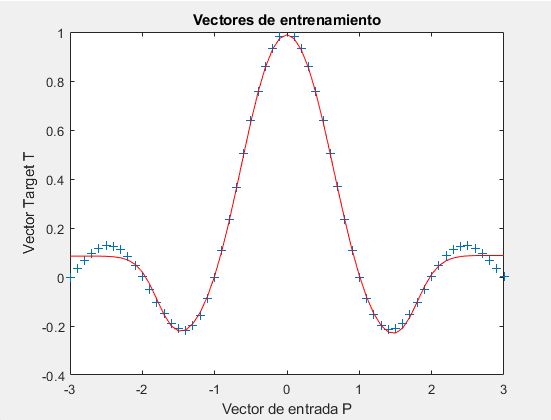
\includegraphics[width=\textwidth]{figures/parte1/Ej2/Ej2_fig3_trainlm.png}
                        \caption{trainlm con 4 neuronas en capa oculta}
                    \end{subfigure}
                    \begin{subfigure}{0.49\textwidth}
                        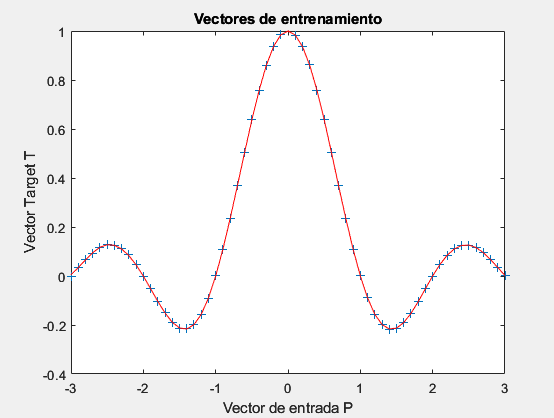
\includegraphics[width=\textwidth]{figures/parte1/Ej2/Ej2_fig7_trainlm_8neuronas.png}
                        \caption{trainlm con 8 neuronas en capa oculta}
                    \end{subfigure}
                \end{figure}

            
            \subsection{Broyden-Fletcher-Goldfarb-Shanno - 'trainbr'}
                Utiliza el algoritmo Broyden-Fletcher-Goldfarb-Shanno (BFGS), una técnica de optimización quasi-Newton. Podemos ver cómo el resultado del entrenamiento con 4 neuronas y con 8 es completamente diferente, pues la primera red no se acerca a la forma de la función y la segunda la aproxima con gran precisión:

                \begin{figure}[htp!]
                    \caption{Levenberg-Marquardt}
                    \begin{subfigure}{0.49\textwidth}
                        \centering
        		      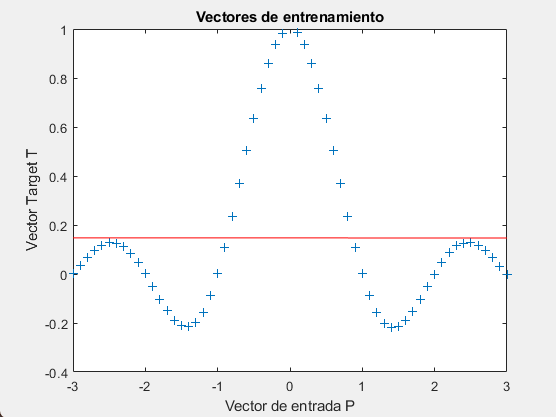
\includegraphics[width=\textwidth]{figures/parte1/Ej2/Ej2_fig4_trainbr.png}
                        \caption{trainbr con 4 neuronas en capa oculta}
                    \end{subfigure}
                    \begin{subfigure}{0.49\textwidth}
                        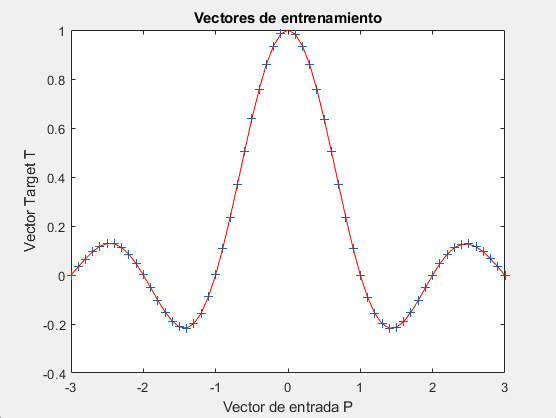
\includegraphics[width=\textwidth]{figures/parte1/Ej2/Ej2_fig8_trainbr_8neuronas.png}
                        \caption{trainbr con 8 neuronas en capa oculta}
                    \end{subfigure}
                \end{figure}

 
        \newpage
        \section{Ejercicio 3. Aproximación de funciones (II).}
            En este ejercicio, se estudiarán en detalle las herramientas que facilita Matlab para el diseño y prueba de redes neuronales ejecutando el siguiente código de ejemplo:

            \inputminted[fontsize=\scriptsize, linenos, breaklines=true, xleftmargin=0.75cm, frame=lines]{matlab}{code/parte1/Ej3.m}

            Explore las gráficas disponibles:
            \begin{enumerate}
                \item Performance: gráfica que representa el error en función del número de épocas para los datos de entrenamiento, validación y test.
                \item Traininig State: evolución del entrenamiento.
                \item Error Histogram: histograma del error.
                \item Regression y Fit: ajuste de los datos de entrenamiento, validación y test.
            \end{enumerate}

            Pruebe este mismo script con el conjunto de datos bodyfat\_dataset, y evalúe sus resultados. Estudie la mejora que supone utilizar distintos métodos de entrenamiento y una división diferente de los datos (entrenamiento, validación y test).

            \newpage
            \subsection{Backpropagation - train}

                Al ejecutar el código con el conjunto de datos bodyfat\_dataset, obtenemos las gráficas de la figura 8. Estas nos proporcionan información útil sobre el entrenamiento. 
                En la figura (a) podemos observar cómo cambia el error de la red con cada grupo de datos en función de las épocas de entrenamiento. Se observa que a partir de la segunda época el error disminuye para los datos del conjunto de entrenamiento, pero aumenta para el de validación, lo cual probablemente sea un ejemplo de sobreajuste de la red a los datos de entrenamiento.

                \begin{figure}[htp!]
                    \caption{Gráficas con Backpropagation}
                    \begin{subfigure}{0.49\textwidth}
                        \centering
        		      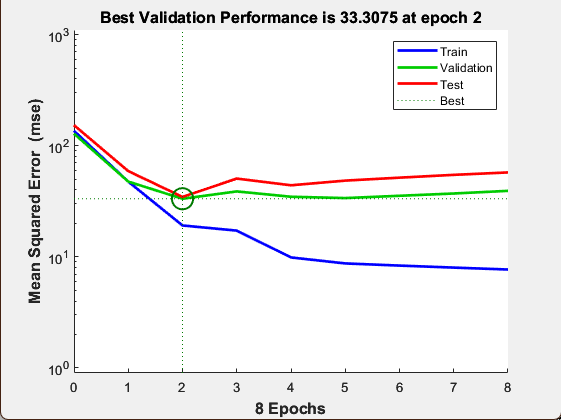
\includegraphics[width=\textwidth]{figures/parte1/Ej3/Ej3_performance_train.png}
                        \caption{Performance con train}
                    \end{subfigure}
                    \begin{subfigure}{0.49\textwidth}
                        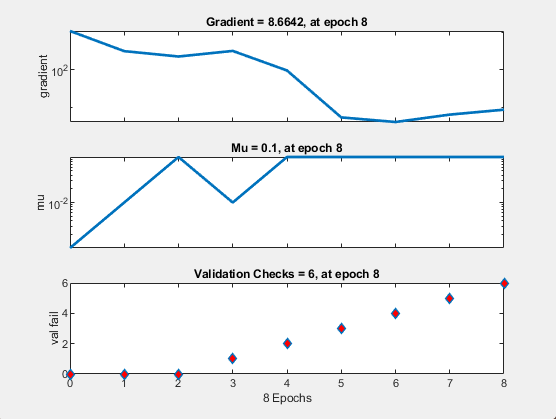
\includegraphics[width=\textwidth]{figures/parte1/Ej3/Ej3_training_state_train.png}
                        \caption{Training state con train}
                    \end{subfigure}
                    \begin{subfigure}{0.49\textwidth}
                        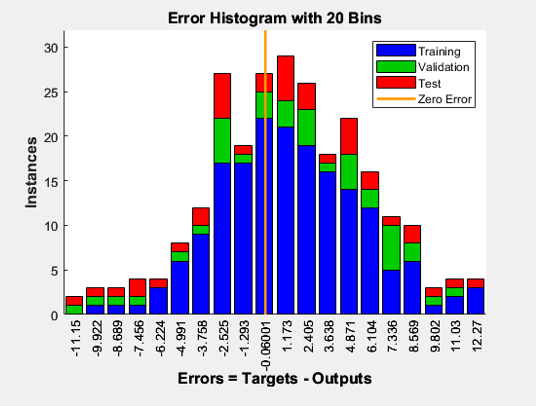
\includegraphics[width=\textwidth]{figures/parte1/Ej3/Ej3_error_train.png}
                        \caption{Error Histogram con train}
                    \end{subfigure}
                    \begin{subfigure}{0.49\textwidth}
                        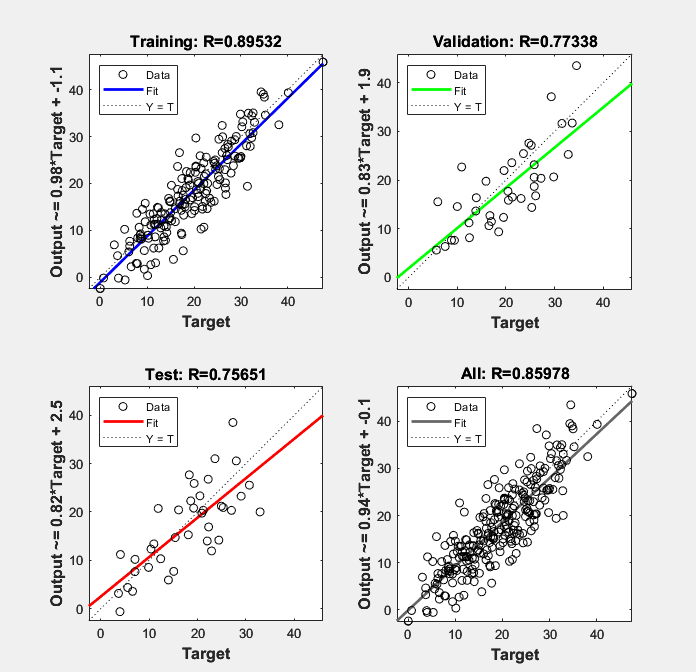
\includegraphics[width=\textwidth]{figures/parte1/Ej3/Ej3_regression_train.png}
                        \caption{Regression con train}
                    \end{subfigure}
                \end{figure}

            \newpage
            \subsection{Backpropagation con división de datos 60/20/20 - train}
                Se ha repetido la ejecución anterior pero con una división diferente de los datos, en este caso hemos pasado de 70/15/15 a 60/20/20. Se puede ver que el punto en el que el mejor rendimiento respecto a los datos de validación ha pasado de ser en la época 6 en lugar de la 2 y una distribución más cercana a cero del error en el histograma. Además de esto no se observan cambios significativos
                \begin{figure}[htp!]
                    \caption{Gráficas con Backpropagation con división 60/20/20}
                    \begin{subfigure}{0.49\textwidth}
                        \centering
        		      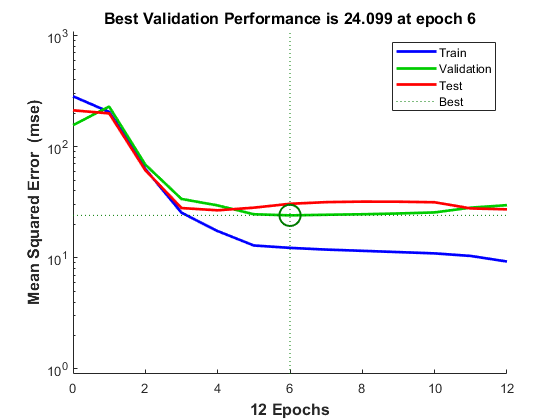
\includegraphics[width=\textwidth]{figures/parte1/Ej3/Ej3_performance_train_60.png}
                        \caption{Performance con train}
                    \end{subfigure}
                    \begin{subfigure}{0.49\textwidth}
                        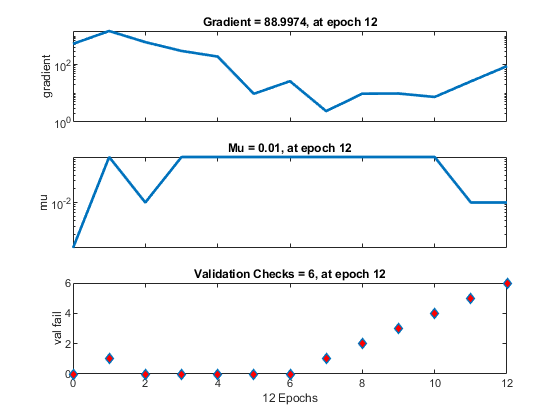
\includegraphics[width=\textwidth]{figures/parte1/Ej3/Ej3_training_state_train_60.png}
                        \caption{Training state con train}
                    \end{subfigure}
                    \begin{subfigure}{0.49\textwidth}
                        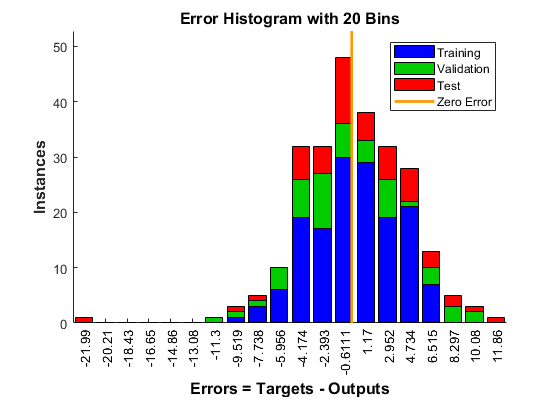
\includegraphics[width=\textwidth]{figures/parte1/Ej3/Ej3_error_train_60.png}
                        \caption{Error Histogram con train}
                    \end{subfigure}
                    \begin{subfigure}{0.49\textwidth}
                        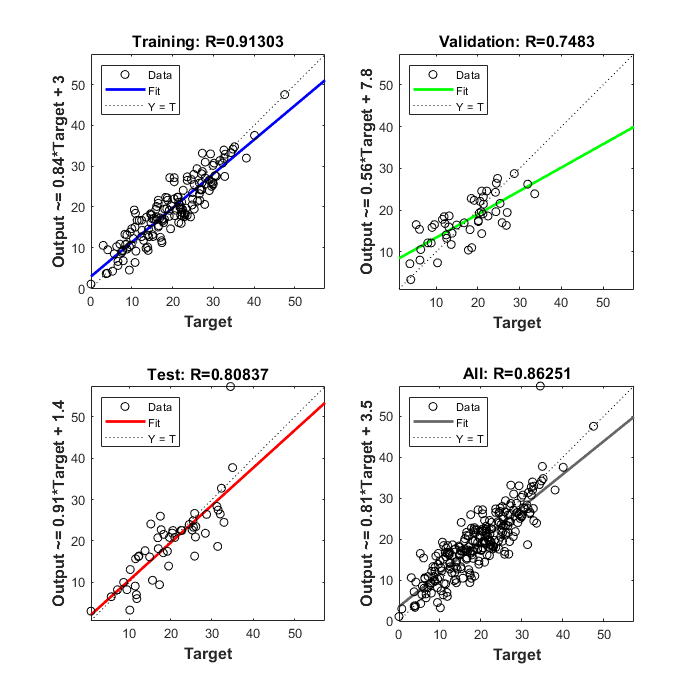
\includegraphics[width=\textwidth]{figures/parte1/Ej3/Ej3_regression_train_60.png}
                        \caption{Regression con train}
                    \end{subfigure}
                \end{figure}

            \newpage
            \subsection{Descenso gradiente con división de datos 70/15/15 - traingd}
                Al repetir el proceso con el método de entrenamiento con descenso gradiente podemos observar que el desempeño empeora con el incremento de las épocas en todos los grupos de datos. También vemos como el error está tan alejado de cero que la línea vertical de ``Zero Error`` ni siquiera aparece en el histograma. Esto sumado al desplazamiento vertical de la línea de regresión respecto a la diagonal (x=y) en la gráfica de regresión nos muestra que la red tiende a realizar una sobreestimación de las predicciones. 
                \begin{figure}[htp!]
                    \caption{Gráficas con Descenso gradiente con división 70/15/15}
                    \begin{subfigure}{0.49\textwidth}
                        \centering
        		      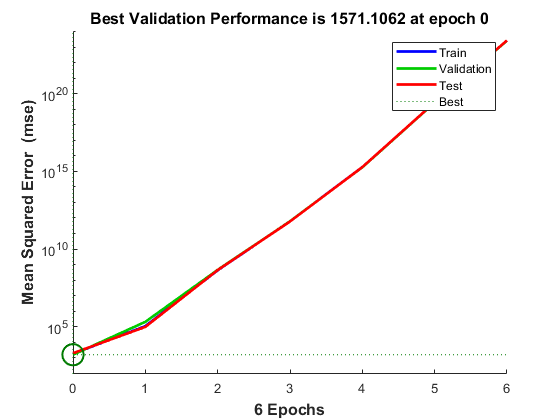
\includegraphics[width=\textwidth]{figures/parte1/Ej3/Ej3_performance_traingd.png}
                        \caption{Performance con traingd}
                    \end{subfigure}
                    \begin{subfigure}{0.49\textwidth}
                        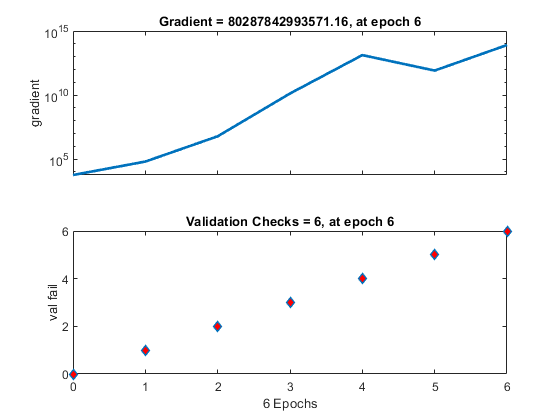
\includegraphics[width=\textwidth]{figures/parte1/Ej3/Ej3_training_state_traingd.png}
                        \caption{Training state con traingd}
                    \end{subfigure}
                    \begin{subfigure}{0.49\textwidth}
                        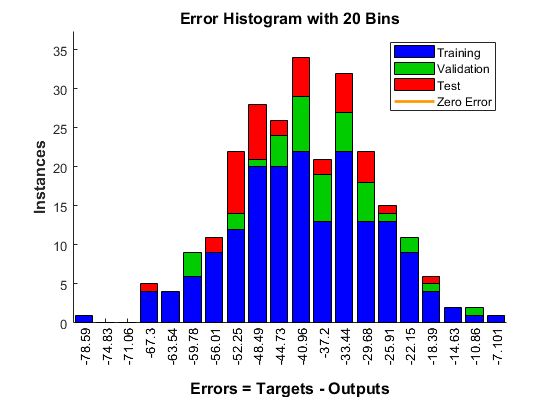
\includegraphics[width=\textwidth]{figures/parte1/Ej3/Ej3_error_traingd.png}
                        \caption{Error Histogram con traingd}
                    \end{subfigure}
                    \begin{subfigure}{0.49\textwidth}
                        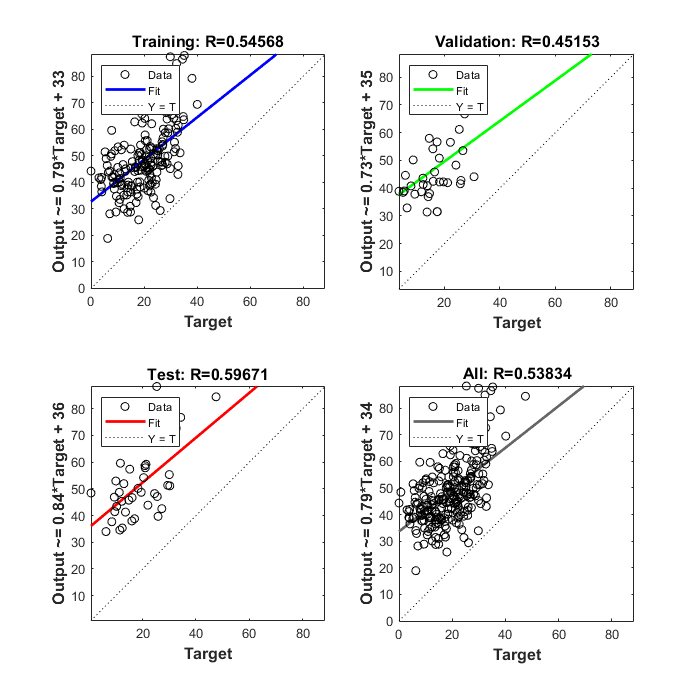
\includegraphics[width=\textwidth]{figures/parte1/Ej3/Ej3_regression_traingd.png}
                        \caption{Regression con traingd}
                    \end{subfigure}
                \end{figure}

            
            \newpage
            \subsection{Descenso gradiente con división de datos 60/20/20 - traingd}
                Al comprobar los resultados de las gráficas con esta división de los datos destaca el cambio abrupto de los valores de los errores en el histograma y de las líneas de regresión anteriormente mencionados. Los valores medios pasan de estar alrededor de -40 a estar entre el 0 y el 20. Las líneas de regresión teniendo una pendiente inferior a 1 también son un indicativo de una subestimación de las predicciones, en contraposición a lo observado con la división 70/15/15.\\ Esta traslación en los valores del error podría indicar que se están realizando divisiones de datos de manera incorrecta o sesgada. Por ejemplo, si los datos de prueba se recopilan de manera que se favorezcan ciertas clases o ejemplos particulares. También se puede observar una aparente dispersión mayor de los datos, aunque esta podría ser un efecto derivado de la escala utilizada en las gráficas variando
                \begin{figure}[htp!]
                    \caption{Gráficas con Descenso gradiente con división 60/20/20}
                    \begin{subfigure}{0.49\textwidth}
                        \centering
        		      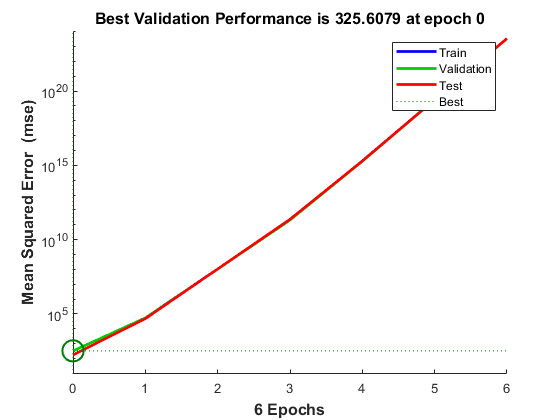
\includegraphics[width=\textwidth]{figures/parte1/Ej3/Ej3_performance_traingd_60.png}
                        \caption{Performance con traingd}
                    \end{subfigure}
                    \begin{subfigure}{0.49\textwidth}
                        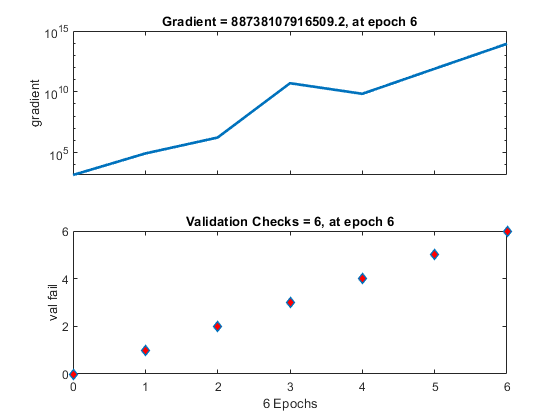
\includegraphics[width=\textwidth]{figures/parte1/Ej3/Ej3_training_state_traingd_60.png}
                        \caption{Training state con traingd}
                    \end{subfigure}
                    \begin{subfigure}{0.49\textwidth}
                        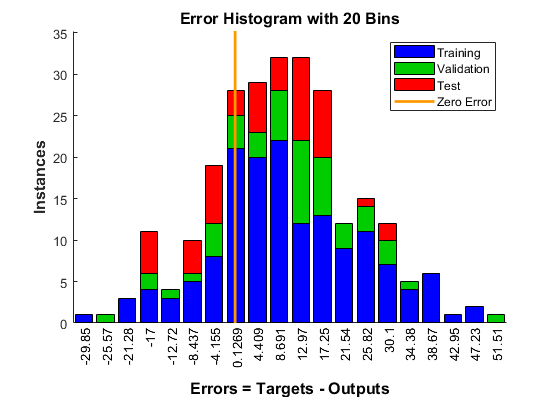
\includegraphics[width=\textwidth]{figures/parte1/Ej3/Ej3_error_traingd_60.png}
                        \caption{Error Histogram con traingd}
                    \end{subfigure}
                    \begin{subfigure}{0.49\textwidth}
                        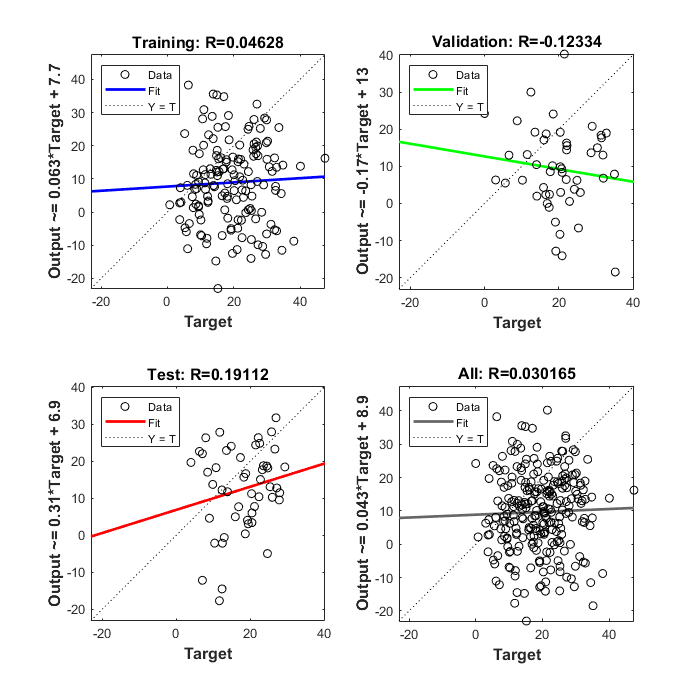
\includegraphics[width=\textwidth]{figures/parte1/Ej3/Ej3_regression_traingd_60.png}
                        \caption{Regression con traingd}
                    \end{subfigure}
                \end{figure}

            \subsection{Levenberg-Marquardt con división de datos 70/15/15 - trainlm}
                Al observar las gráficas obtenidas de aplicar este método de entrenamiento, destacan el gran incremento en las épocas de entrenamiento (10 más que el mayor realizado con los otros métodos) y un descenso abrupto en los "validation checks" después de un número específico de épocas, en este caso, después de 16 épocas. Esto indica una mejora significativa en el rendimiento del modelo de aprendizaje durante ese período, además, coincide con la época de mejor rendimiento en el conjunto de validación
                \begin{figure}[htp!]
                    \caption{Gráficas con Levenberg-Marquardt con división 70/15/15}
                    \begin{subfigure}{0.49\textwidth}
                        \centering
        		      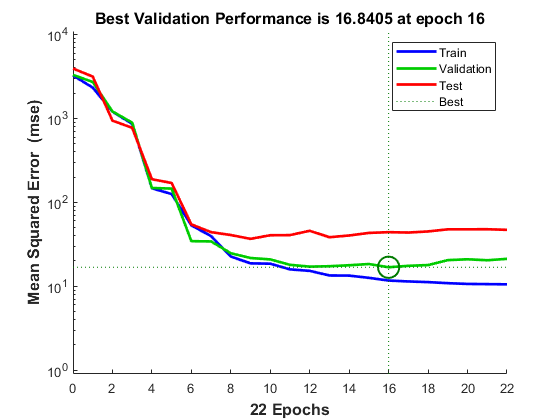
\includegraphics[width=\textwidth]{figures/parte1/Ej3/Ej3_performance_trainlm.png}
                        \caption{Performance con trainlm}
                    \end{subfigure}
                    \begin{subfigure}{0.49\textwidth}
                        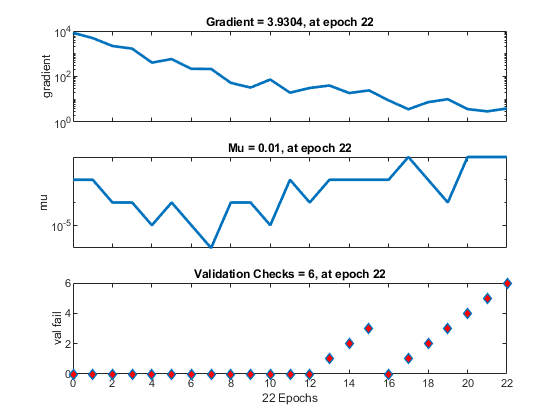
\includegraphics[width=\textwidth]{figures/parte1/Ej3/Ej3_training_state_trainlm.png}
                        \caption{Training state con trainlm}
                    \end{subfigure}
                    \begin{subfigure}{0.49\textwidth}
                        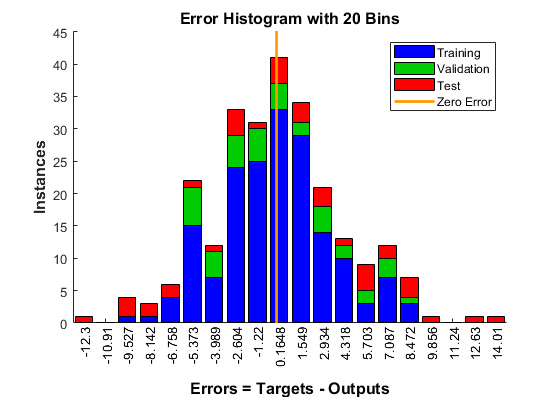
\includegraphics[width=\textwidth]{figures/parte1/Ej3/Ej3_error_trainlm.png}
                        \caption{Error Histogram con trainlm}
                    \end{subfigure}
                    \begin{subfigure}{0.49\textwidth}
                        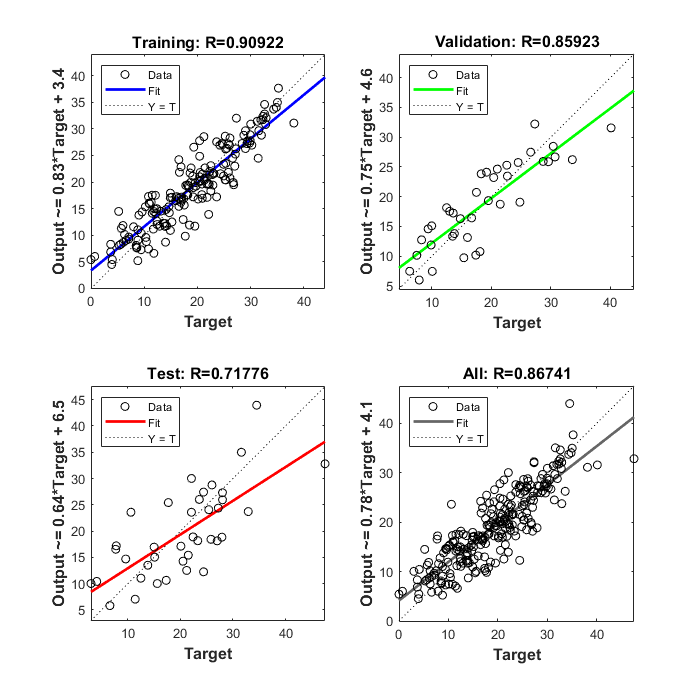
\includegraphics[width=\textwidth]{figures/parte1/Ej3/Ej3_regression_trainlm.png}
                        \caption{Regression con trainlm}
                    \end{subfigure}
                \end{figure}

            
            \newpage
            \subsection{Levenberg-Marquardt con división de datos 60/20/20 - train}
                Al repetirse la ejecución anterior pero con una división diferente de los datos, el resultado es aparentemente peor pero más rápido, ya que el mejor rendimiento aparece después de 6 épocas, siendo mayor el grado de error comparado a la ejecución anterior. Podemos observar que a partir de esta época la red muestra signos de sobreajuste, por lo que podría intuirse que un grupo de datos de entrenamiento de mayor tamaño es más apropiado para redes entrenadas con este algoritmo.
                \begin{figure}[htp!]
                    \caption{Gráficas con Levenberg-Marquardt con división 60/20/20}
                    \begin{subfigure}{0.49\textwidth}
                        \centering
        		      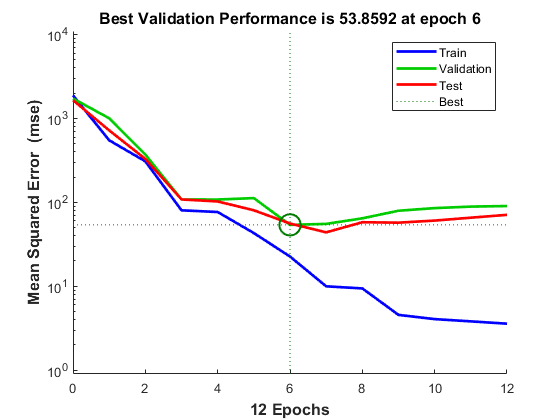
\includegraphics[width=\textwidth]{figures/parte1/Ej3/Ej3_performance_trainlm_60.png}
                        \caption{Performance con trainlm}
                    \end{subfigure}
                    \begin{subfigure}{0.49\textwidth}
                        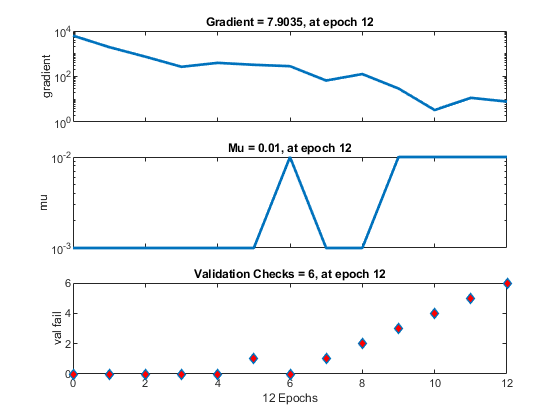
\includegraphics[width=\textwidth]{figures/parte1/Ej3/Ej3_training_state_trainlm_60.png}
                        \caption{Training state con trainlm}
                    \end{subfigure}
                    \begin{subfigure}{0.49\textwidth}
                        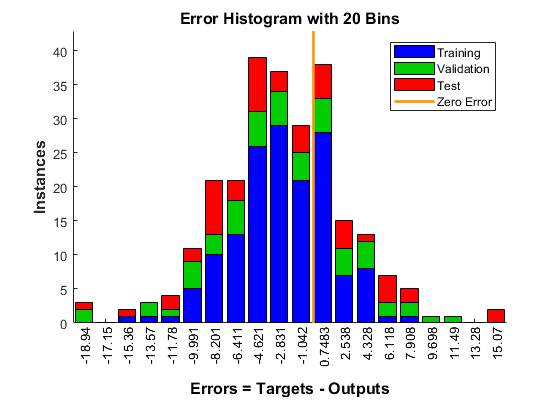
\includegraphics[width=\textwidth]{figures/parte1/Ej3/Ej3_error_trainlm_60.png}
                        \caption{Error Histogram con trainlm}
                    \end{subfigure}
                    \begin{subfigure}{0.49\textwidth}
                        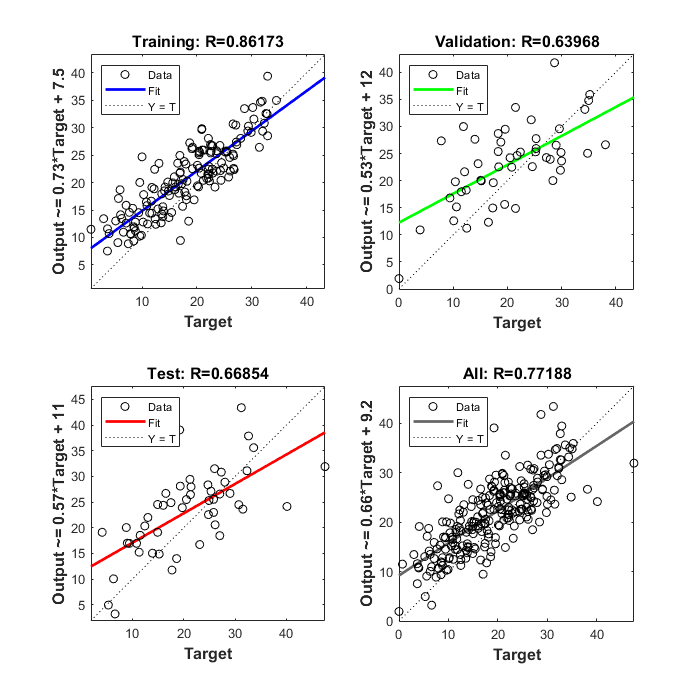
\includegraphics[width=\textwidth]{figures/parte1/Ej3/Ej3_regression_trainlm_60.png}
                        \caption{Regression con trainlm}
                    \end{subfigure}
                \end{figure}

        
        \newpage
        \section{Ejercicio 4. Clasificación.}
            La clasificación de patrones es una de las aplicaciones que dieron origen a las redes neuronales artificiales. Como en el caso anterior, la toolbox de redes neuronales de Matlab dispone de una red optimizada para la clasificación, patternnet, que analizaremos en este ejemplo. De estos resultados cabe destacar que no ha habido ningún falso negativo en las predicciones de validación.

            \inputminted[fontsize=\scriptsize, linenos, breaklines=true, xleftmargin=0.75cm, frame=lines]{matlab}{code/parte1/Ej4.m}

            En lugar de las gráficas específicamente relacionadas con la aproximación de una función, en el caso de una tarea de clasificación, se ofrecen:
            \begin{enumerate}
                \item Confusion: matrices de confusión de los resultados.
                \item Receiver Operating Charactersitic: curvas ROC (característica operativa del receptor).
            \end{enumerate}

            Pruebe este mismo script con el conjunto de datos cancer\_dataset, y evalúe sus resultados. Estudie de nuevo la mejora que supone utilizar distintos métodos de entrenamiento y una división diferente de los datos (entrenamiento, validación y test).

            \newpage
            \subsection{Backpropagation}
                La matriz de confusión y gráfica de ROC obtenidas al entrenar la red con el algoritmo de backpropagation en el conjunto de datos cancer\_dataset muestran la proporción de verdaderos positivos, verdaderos negativos, falsos positivos y falsos negativos. Los resultados obtenidos son relativamente buenos, ya que la precisión más baja en es de un 95.7\% y el área bajo la curva en la gráfica Receiver Operating Charactersitic supone una gran parte (si no toda) del área total. Los resultados positivos se repiten con tódos los métodos de entrenamiento probados, con ligeras variaciones en función de la división de los datos.

                \begin{figure}[htp!]
                    \caption{Gráficas con Backpropagation con división 70/15/15}
                    \begin{subfigure}{0.49\textwidth}
                        \centering
        		      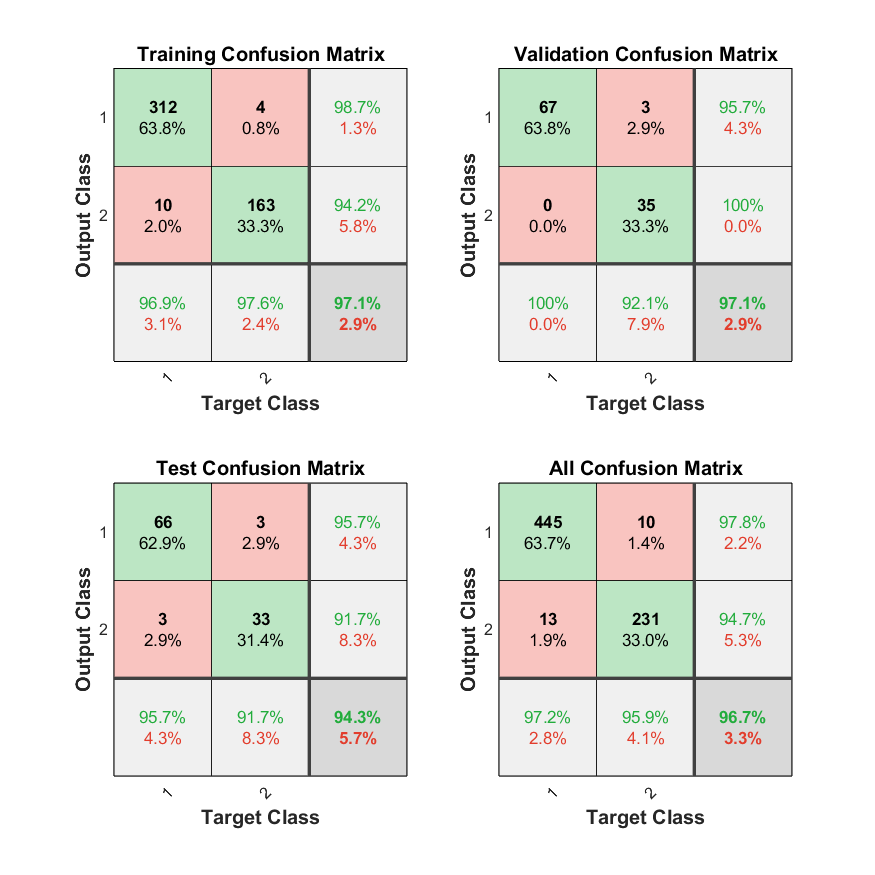
\includegraphics[width=\textwidth]{figures/parte1/Ej4/ej4_confusion_train.png}
                        \caption{Confusion con train}
                    \end{subfigure}
                    \begin{subfigure}{0.49\textwidth}
                        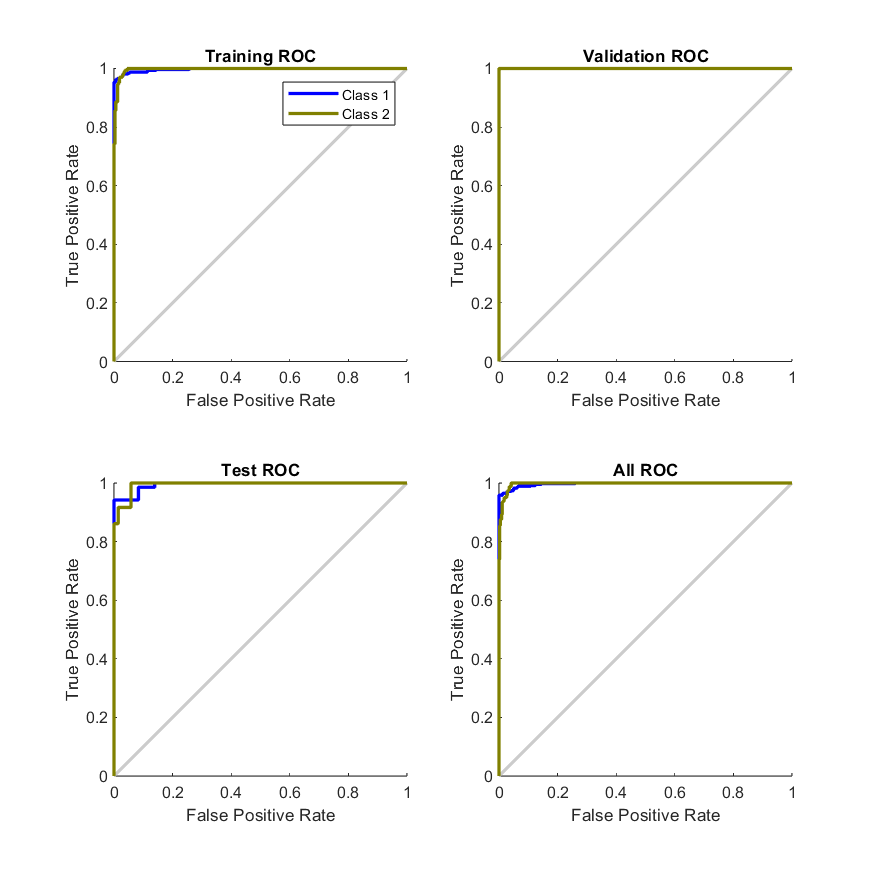
\includegraphics[width=\textwidth]{figures/parte1/Ej4/ej4_roc_train.png}
                        \caption{Receiver Operating Charactersitic con train}
                    \end{subfigure}
                \end{figure}

            \newpage
            \subsection{Backpropagation con división de datos 60/20/20}
                Al cambiar la división de los datos se observa un resultado ligeramente peor en la matriz ``All Confusion Matrix``, al igual que en la de validación. Ahora sí que hay falsos negativos en las predicciones de validación. Por lo demás los resultados son muy similares.
                \begin{figure}[htp!]
                    \caption{Gráficas con Backpropagation con división 60/20/20}
                    \begin{subfigure}{0.49\textwidth}
                        \centering
        		      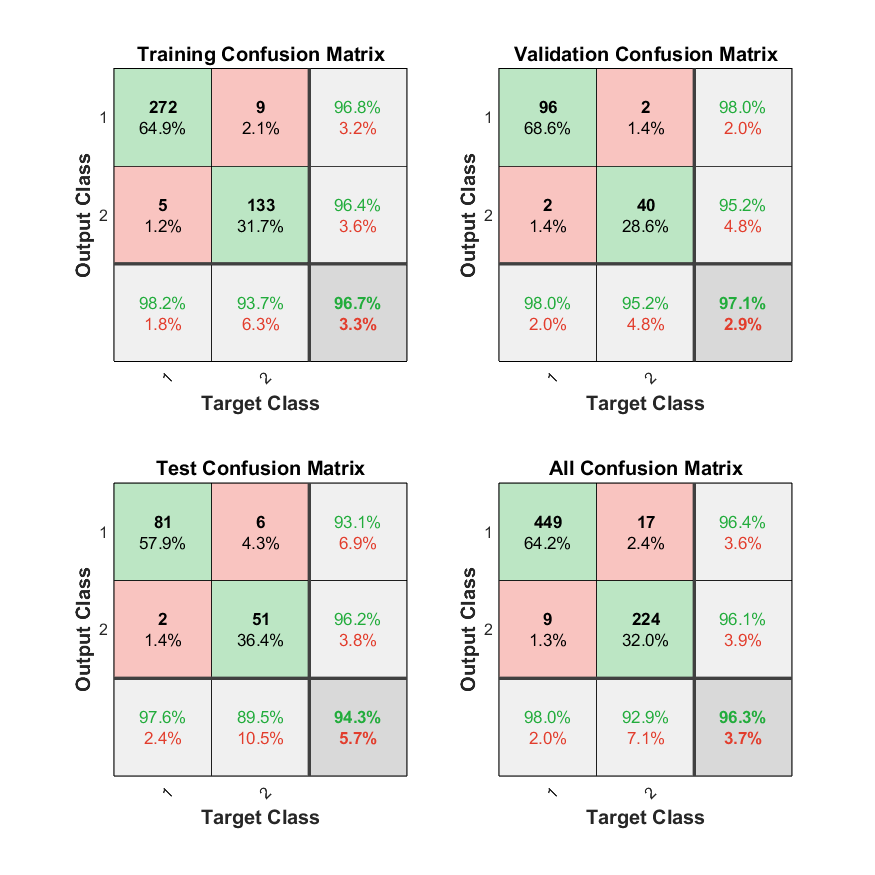
\includegraphics[width=\textwidth]{figures/parte1/Ej4/ej4_confusion_train_60.png}
                        \caption{Confusion con train}
                    \end{subfigure}
                    \begin{subfigure}{0.49\textwidth}
                        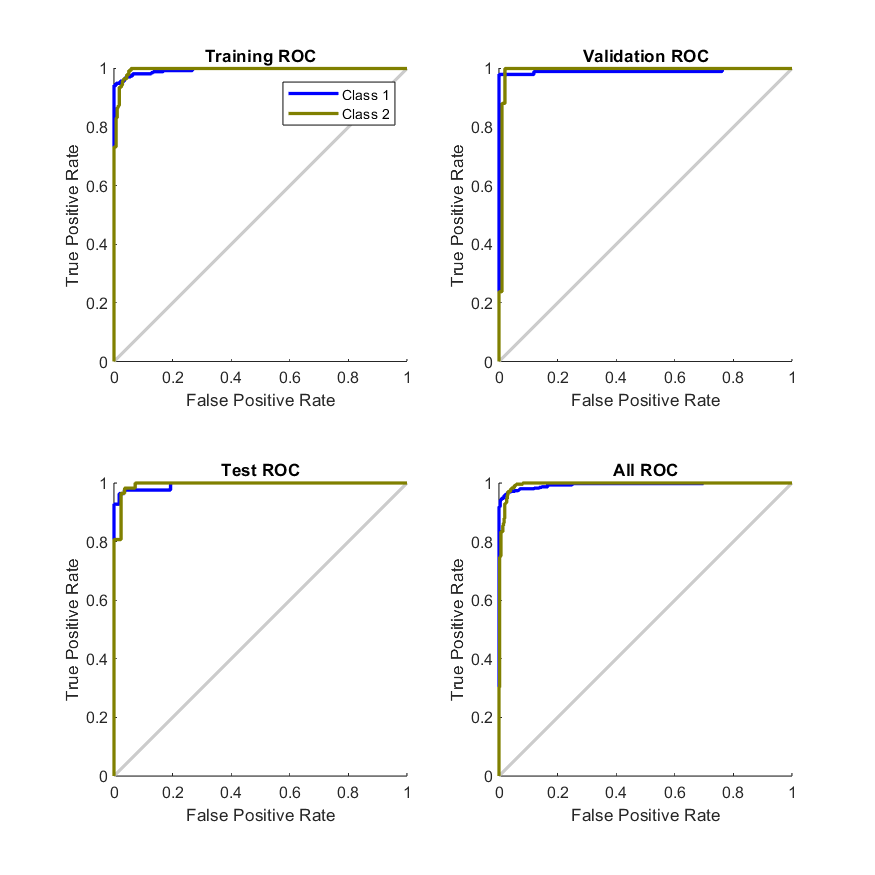
\includegraphics[width=\textwidth]{figures/parte1/Ej4/ej4_roc_train_60.png}
                        \caption{Receiver Operating Charactersitic con train}
                    \end{subfigure}
                \end{figure}

            \newpage
            \subsection{Descenso gradiente}
                Las gráficas de la red entrenada con descenso gradiente muestran un resultado ligeramente peor a las entrenadas con backpropagation
                \begin{figure}[htp!]
                    \caption{Gráficas con Descenso gradiente con división 70/15/15}
                    \begin{subfigure}{0.49\textwidth}
                        \centering
        		      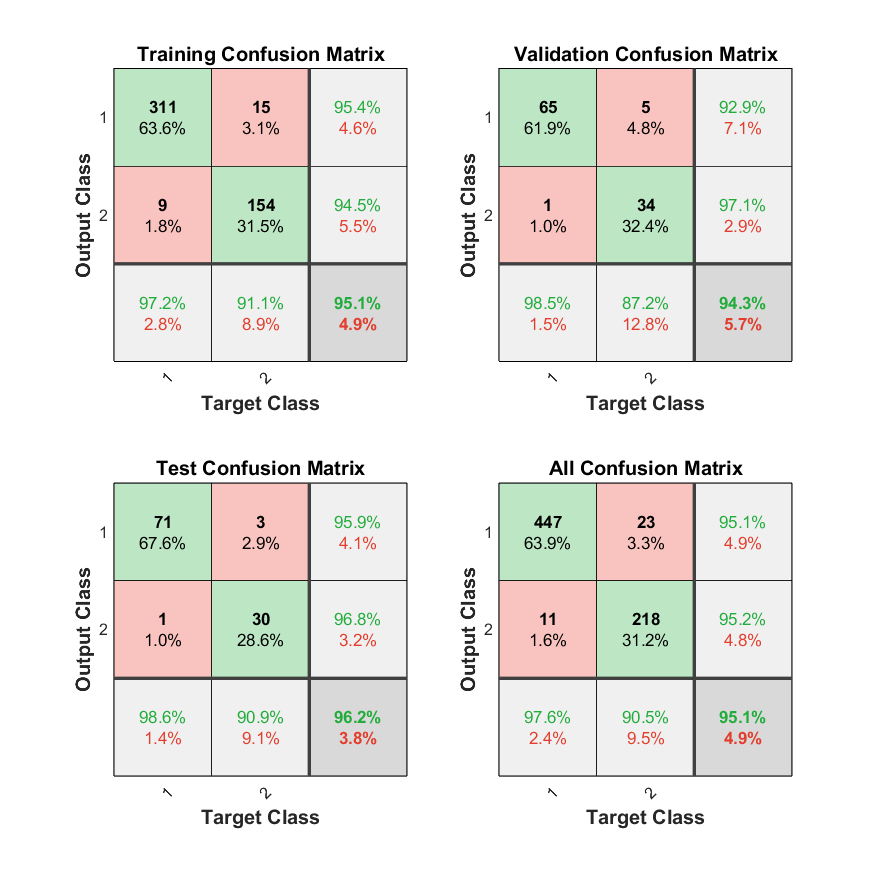
\includegraphics[width=\textwidth]{figures/parte1/Ej4/ej4_confusion_traingd.png}
                        \caption{Confusion con traingd}
                    \end{subfigure}
                    \begin{subfigure}{0.49\textwidth}
                        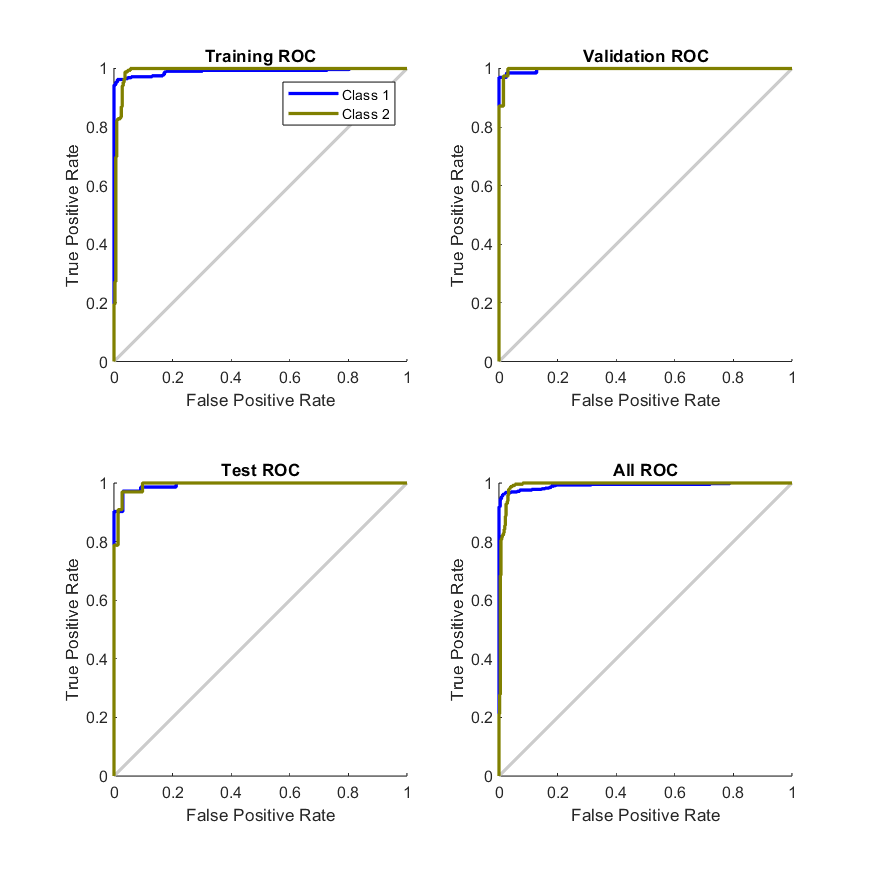
\includegraphics[width=\textwidth]{figures/parte1/Ej4/ej4_roc_traingd.png}
                        \caption{Receiver Operating Charactersitic con traingd}
                    \end{subfigure}
                \end{figure}

            \newpage
            \subsection{Descenso gradiente con división de datos 60/20/20}
                Se ha repetido la ejecución anterior pero con una división diferente de los datos. El resultado en las predicciones de validación mejora en cuanto a precisión pero empeora en cuanto a sensibilidad. En conjunto resulta muy similar.
                \begin{figure}[htp!]
                    \caption{Gráficas con Descenso gradiente con división 60/20/20}
                    \begin{subfigure}{0.49\textwidth}
                        \centering
        		      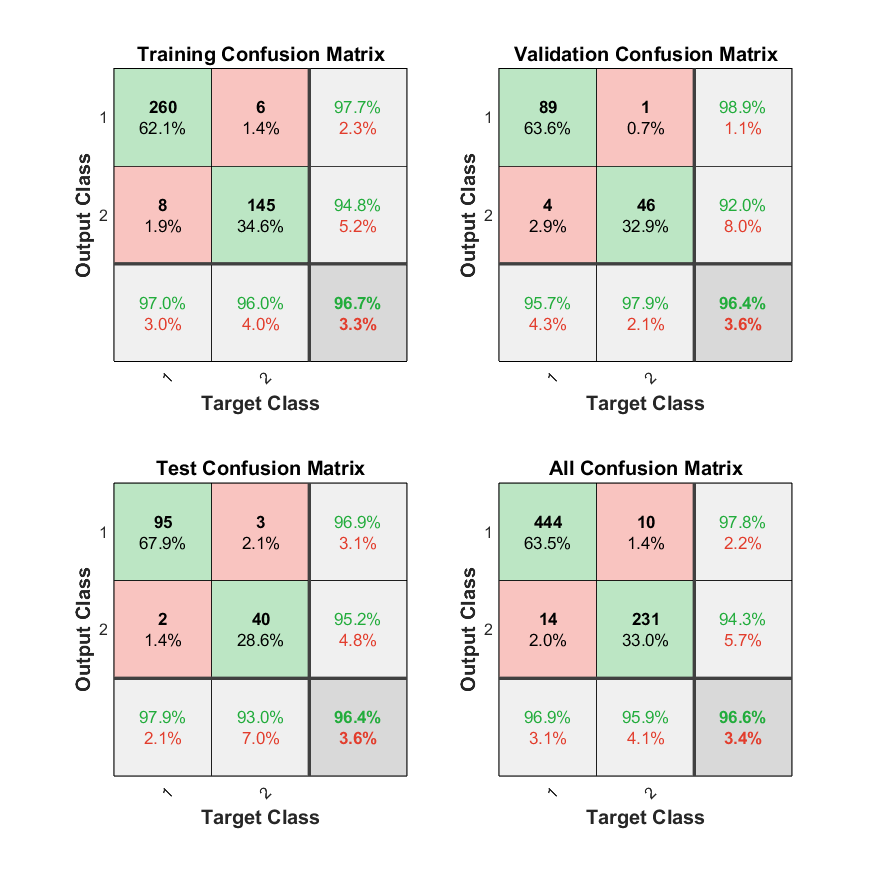
\includegraphics[width=\textwidth]{figures/parte1/Ej4/ej4_confusion_traingd_60.png}
                        \caption{Confusion con traingd}
                    \end{subfigure}
                    \begin{subfigure}{0.49\textwidth}
                        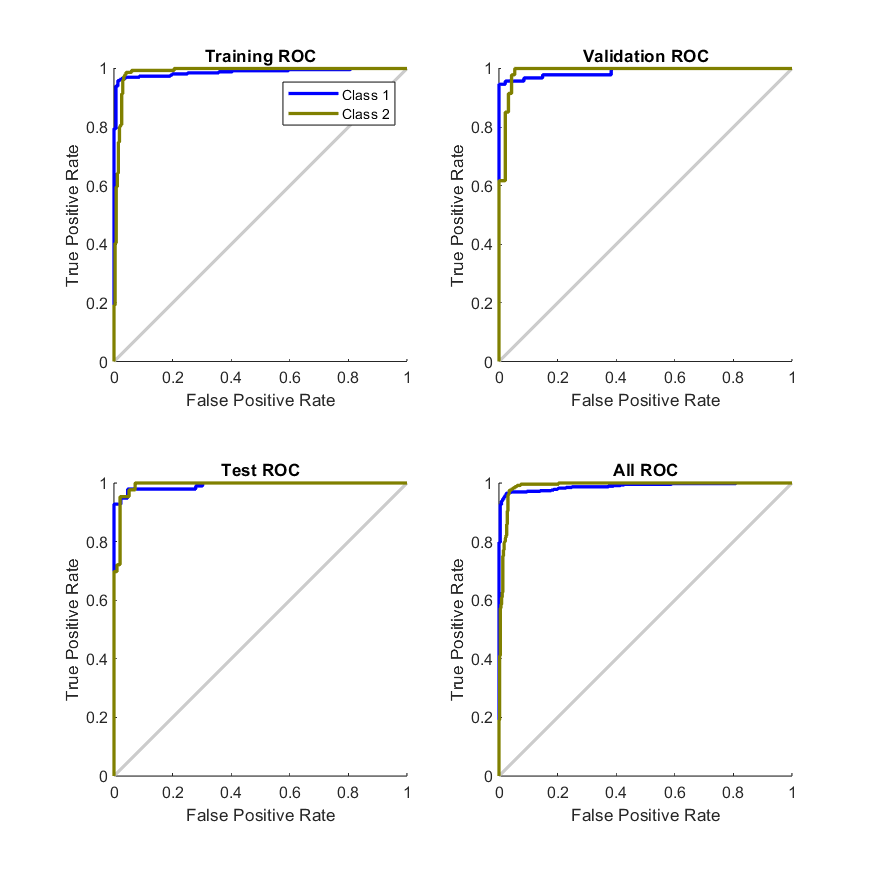
\includegraphics[width=\textwidth]{figures/parte1/Ej4/ej4_roc_traingd_60.png}
                        \caption{Receiver Operating Charactersitic con traingd}
                    \end{subfigure}
                \end{figure}

            \newpage
            \subsection{Levenberg-Marquardt}
                La Matriz de confusión y las gráficas ROC muestran resultados muy similares con este algoritmo también. Aparentemente todos los métodos probados son bastante buenos en cuanto a clasificación. 
                \begin{figure}[htp!]
                    \caption{Gráficas con Levenberg-Marquardt con división 70/15/15}
                    \begin{subfigure}{0.49\textwidth}
                        \centering
        		      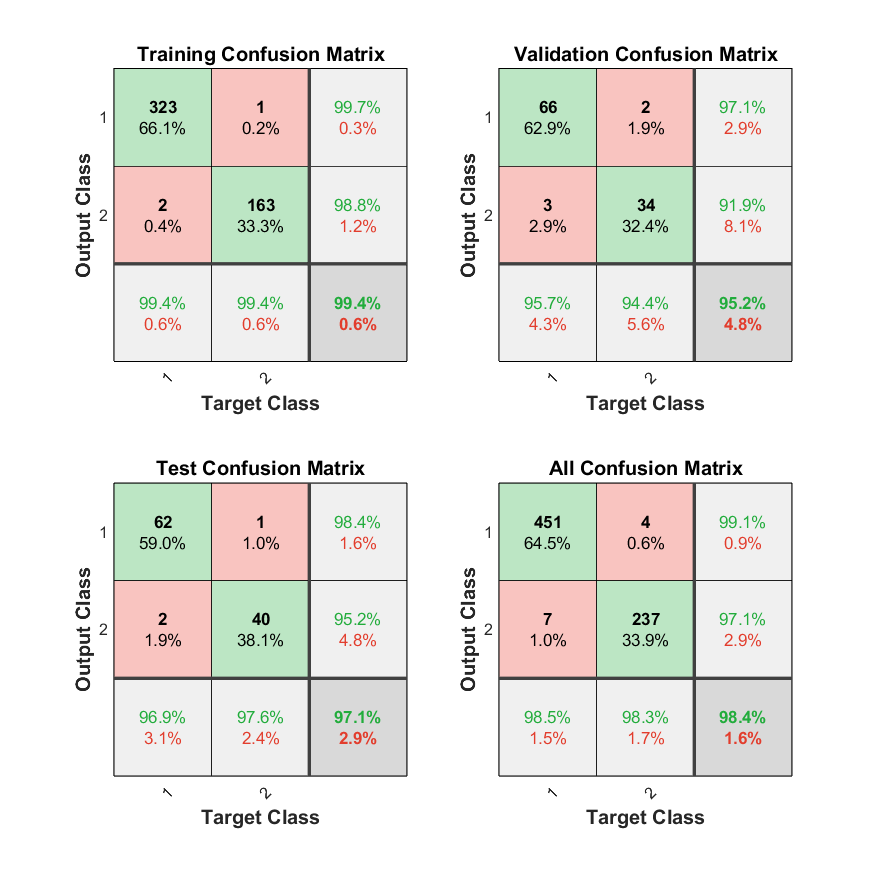
\includegraphics[width=\textwidth]{figures/parte1/Ej4/ej4_confusion_trainlm.png}
                        \caption{Confusion con train}
                    \end{subfigure}
                    \begin{subfigure}{0.49\textwidth}
                        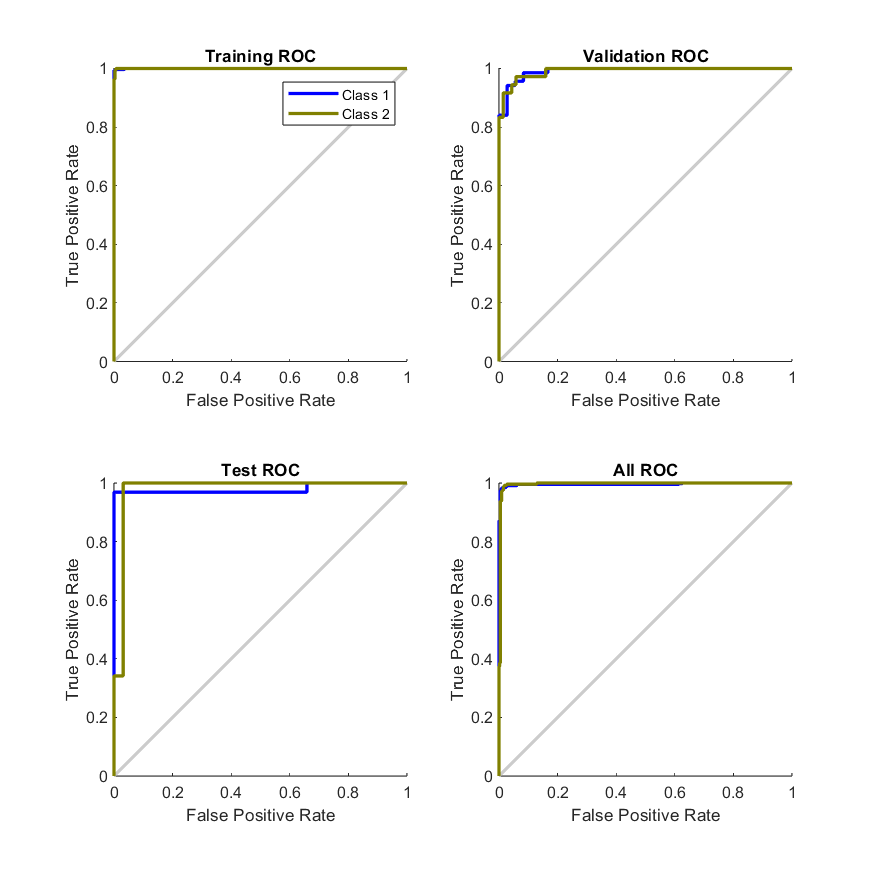
\includegraphics[width=\textwidth]{figures/parte1/Ej4/ej4_roc_trainlm.png}
                        \caption{Receiver Operating Charactersitic con trainlm}
                    \end{subfigure}
                \end{figure}

            \newpage
            \subsection{Gráficas con Levenberg-Marquardt con división 60/20/20}
                Esta última matriz de confusión no presenta ningún falso negativo (al igual que backpropagation con 70/15/15) en las predicciones de validación a pesar del aumento en la cantidad de datos en este grupo respecto a la prueba anterior. Esto no representa un cambio significativo respecto al resto de pruebas (las cuales presentaban entre 0 y 4 falsos negativos en este área)
                \begin{figure}[htp!]
                    \caption{Gráficas con Levenberg-Marquardt con división 60/20/20}
                    \begin{subfigure}{0.49\textwidth}
                        \centering
        		      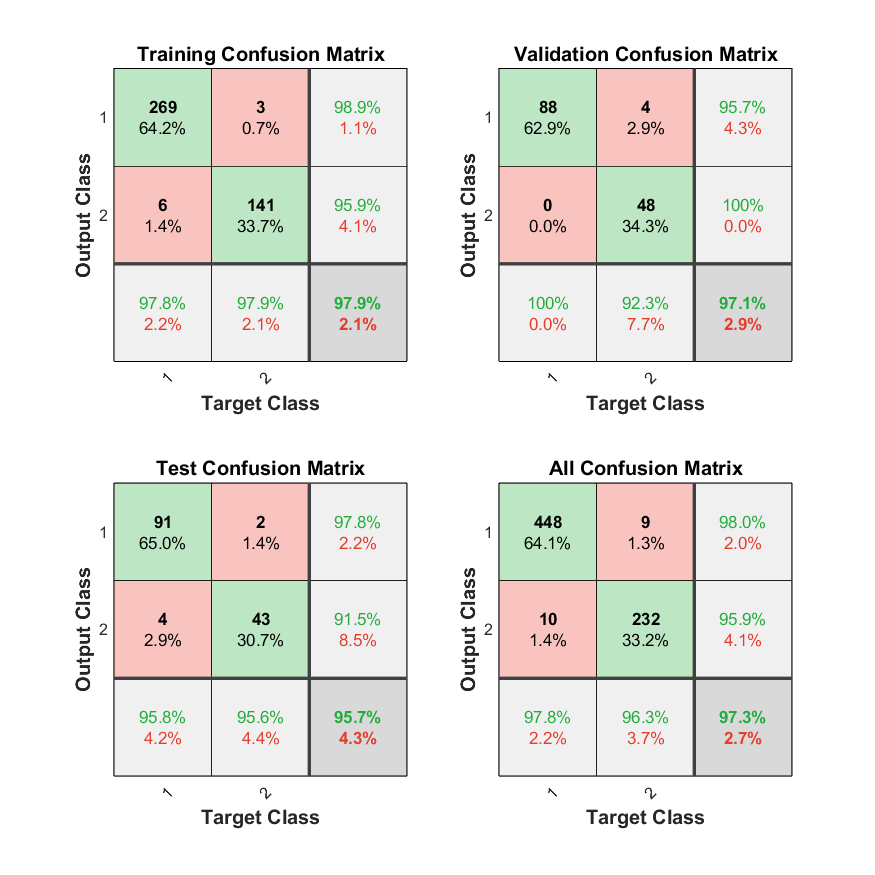
\includegraphics[width=\textwidth]{figures/parte1/Ej4/ej4_confusion_trainlm_60.png}
                        \caption{Confusion con trainlm}
                    \end{subfigure}
                    \begin{subfigure}{0.49\textwidth}
                        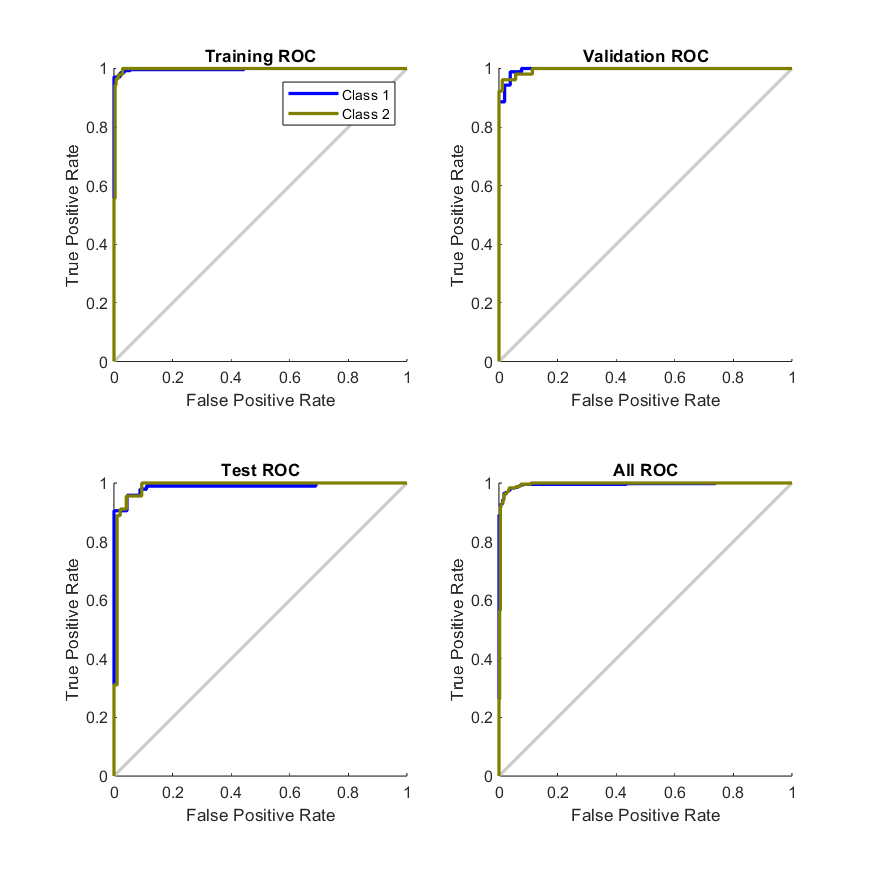
\includegraphics[width=\textwidth]{figures/parte1/Ej4/ej4_roc_trainlm_60.png}
                        \caption{Receiver Operating Charactersitic con trainlm}
                    \end{subfigure}
                \end{figure}
                \newpage
                
	\part{Diseño de un control de posición mediante una red neuronal no recursiva.}
	
	\section{Desarrollo}
	
	\subsection{Esquema de Simulink}
		\begin{figure}[htp!]
			\centering
			\includegraphics[width=1\textwidth]{figures/parte2/ejerA.png}
			\caption{Esquema general Simulink.}
		\end{figure}
		
	\subsection{Creaación script para simular el diagrama.}
		\inputminted[fontsize=\scriptsize, linenos, breaklines=true, xleftmargin=0.75cm, frame=lines]{matlab}{code/parte2/EjerB.m}
	
	\newpage
	\subsection{Ejecución script y comprobación de variables.}
		Podemos observar que se generan las variables que contienen las salidas y entradas del controlador y las salidas del robot durante la simulación correctamente.
		\begin{figure}[htp!]
			\centering
			\includegraphics[width=0.4\textwidth]{figures/parte2/ejerC.png}
			\caption{Variables.}
		\end{figure}
	
	\newpage
	\subsection{Trayectoria del robot.}
		\inputminted[fontsize=\scriptsize, linenos, breaklines=true, xleftmargin=0.75cm, frame=lines]{matlab}{code/parte2/EjerD.m}
		Podemos ver la trayectoria que sigue el robot en la siguiente gráfica:
		\begin{figure}[htp!]
			\centering
			\includegraphics[width=0.8\textwidth]{figures/parte2/ejerD.jpg}
			\caption{Trayectoria del robot.}
		\end{figure}
	\newpage
	
	\subsection{Generar N posiciones aleatorias, simular y guardar en variables.}
		\inputminted[fontsize=\scriptsize, linenos, breaklines=true, xleftmargin=0.75cm, frame=lines]{matlab}{code/parte2/EjerE.m}
		
	\subsection{Entrenamiento de red neuronal con 10 neuronas en la capa oculta.}
		\inputminted[fontsize=\scriptsize, linenos, breaklines=true, xleftmargin=0.75cm, frame=lines]{matlab}{code/parte2/EjerF.m}
		
		\begin{figure}[htp!]
			\centering
			\includegraphics[width=0.4\textwidth]{figures/parte2/ejerF.png}
			\caption{Resultados del entrenamiento.}
		\end{figure}
	\newpage
	\subsection{Generación de bloque de Simulink con el controlador neuronal.}
		\inputminted[fontsize=\scriptsize, linenos, breaklines=true, xleftmargin=0.75cm, frame=lines]{matlab}{code/parte2/EjerG.m}
		
		\begin{figure}[htp!]
			\centering
			\includegraphics[width=0.6\textwidth]{figures/parte2/ejerG.png}
			\caption{Bloque simulado por gensim.}
		\end{figure}
	
	\subsection{Esquema de Simulink con la red neuronal en lugar del bloque controlador.}
	Tras sustituir el bloque controlador por el bloque generado, la figura queda de la siguiente forma:
	\begin{figure}[htp!]
		\centering
		\includegraphics[width=1\textwidth]{figures/parte2/ejerH.png}
		\caption{Esquema del controlador neuronal de posición.}
	\end{figure}
	
	\newpage
	\subsection{Comparación.}
	Se ha hecho el siguiente código para estudiar las diferencias entre los comportamientos y el error que conlleva.
	\inputminted[fontsize=\scriptsize, linenos, breaklines=true, xleftmargin=0.75cm, frame=lines]{matlab}{code/parte2/compararComportamiento.m}
	\newpage
	Podemos observar que las trayectorias son bastantes parecidas y los  errores no son demasiado grandes en las siguientes gráficas
	\begin{figure}[htp!]
		\centering
		\includegraphics[width=0.8\textwidth]{figures/parte2/ejerI.png}
		\caption{Gráficos para comparar trayectorias entre los dos esquemas.}
	\end{figure}
	
	Tras varias pruebas el error medio varía entre los siguientes valores:
	\begin{figure}[htp!]
		\centering
		\includegraphics[width=0.4\textwidth]{figures/parte2/ejerI2.png}
		\caption{Errores medios de varias ejecuciones.}
	\end{figure}
	
	Podemos concluir que los errores no son demasiado significativos y que están en un rango esperado.
	
 \end{document}
